% $Id: template.tex 11 2007-04-03 22:25:53Z jpeltier $

\documentclass{vgtc}
% final (conference style)
%\documentclass[review]{vgtc}                 % review
%\documentclass[widereview]{vgtc}             % wide-spaced review
%\documentclass[preprint]{vgtc}               % preprint
%\documentclass[electronic]{vgtc}             % electronic version

%% Uncomment one of the lines above depending on where your paper is
%% in the conference process. ``review'' and ``widereview'' are for review
%% submission, ``preprint'' is for pre-publication, and the final version
%% doesn't use a specific qualifier. Further, ``electronic'' includes
%% hyperreferences for more convenient online viewing.

%% Please use one of the ``review'' options in combination with the
%% assigned online id (see below) ONLY if your paper uses a double blind
%% review process. Some conferences, like IEEE Vis and InfoVis, have NOT
%% in the past.

%% Figures should be in CMYK or Grey scale format, otherwise, colour 
%% shifting may occur during the printing process.

%% These few lines make a distinction between latex and pdflatex calls and they
%% bring in essential packages for graphics and font handling.
%% Note that due to the \DeclareGraphicsExtensions{} call it is no longer necessary
%% to provide the the path and extension of a graphics file:
%% \includegraphics{diamondrule} is completely sufficient.
%%
\ifpdf%                                % if we use pdflatex
  \pdfoutput=1\relax                   % create PDFs from pdfLaTeX
  \pdfcompresslevel=9                  % PDF Compression
  \pdfoptionpdfminorversion=7          % create PDF 1.7
  \ExecuteOptions{pdftex}
  \usepackage{graphicx}                % allow us to embed graphics files
  \DeclareGraphicsExtensions{.pdf,.png,.jpg,.jpeg} % for pdflatex we expect .pdf, .png, or .jpg files
\else%                                 % else we use pure latex
  \ExecuteOptions{dvips}
  \usepackage{graphicx}                % allow us to embed graphics files
  \DeclareGraphicsExtensions{.eps}     % for pure latex we expect eps files
\fi%

%% it is recomended to use ``\autoref{sec:bla}'' instead of ``Fig.~\ref{sec:bla}''
\graphicspath{{figures/}{pictures/}{images/}{./}} % where to search for the images

\usepackage{microtype}                 % use micro-typography (slightly more compact, better to read)
\PassOptionsToPackage{warn}{textcomp}  % to address font issues with \textrightarrow
\usepackage{textcomp}                  % use better special symbols
\usepackage{amsmath}                  % use matching math font
\usepackage{times}                     % we use Times as the main font
\renewcommand*\ttdefault{txtt}         % a nicer typewriter font
\usepackage{cite}                      % needed to automatically sort the references
\usepackage{tabu}                      % only used for the table example
\usepackage{booktabs}                  % only used for the table example
%% We encourage the use of mathptmx for consistent usage of times font
%% throughout the proceedings. However, if you encounter conflicts
%% with other math-related packages, you may want to disable it.


%% If you are submitting a paper to a conference for review with a double
%% blind reviewing process, please replace the value ``0'' below with your
%% OnlineID. Otherwise, you may safely leave it at ``0''.
\onlineid{0}

%% declare the category of your paper, only shown in review mode
\vgtccategory{Research}

%% allow for this line if you want the electronic option to work properly
\vgtcinsertpkg

%% In preprint mode you may define your own headline.
%\preprinttext{To appear in an IEEE VGTC sponsored conference.}

%% Paper title.

\title{Drumming in VR - A Case Study}

%% This is how authors are specified in the conference style

%% Author and Affiliation (single author).
%%\author{Roy G. Biv\thanks{e-mail: roy.g.biv@aol.com}}
%%\affiliation{\scriptsize Allied Widgets Research}

%% Author and Affiliation (multiple authors with single affiliations).
%%\author{Roy G. Biv\thanks{e-mail: roy.g.biv@aol.com} %
%%\and Ed Grimley\thanks{e-mail:ed.grimley@aol.com} %
%%\and Martha Stewart\thanks{e-mail:martha.stewart@marthastewart.com}}
%%\affiliation{\scriptsize Martha Stewart Enterprises \\ Microsoft Research}

%% Author and Affiliation (multiple authors with multiple affiliations)
\author{Anca-Simona Horvath\thanks{e-mail: ancah@hum.aau.dk}\\ %
        \scriptsize Humanities, AAU %
\and Mauro Nascimben \thanks{e-mail: mana@create.aau.dk}\\ %
     \scriptsize CREATE, AAU CPH %
\and Silvin Willemsen\thanks{e-mail: sil@create.aau.dk}\\ %
     \parbox{1.4in}{\scriptsize \centering Multisensory Experience Lab \\ CREATE, AAU CPH}}

%% A teaser figure can be included as follows, but is not recommended since
%% the space is now taken up by a full width abstract.
%\teaser{
%  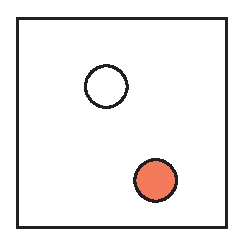
\includegraphics[width=1.5in]{sample.eps}
%  \caption{Lookit! Lookit!}
%}

%% Abstract section.
\abstract{Duis autem vel eum iriure dolor in hendrerit in vulputate
velit esse molestie consequat, vel illum dolore eu feugiat nulla
facilisis at vero eros et accumsan et iusto odio dignissim qui blandit
praesent luptatum zzril delenit augue duis dolore te feugait nulla
facilisi. Lorem ipsum dolor sit amet, consectetuer adipiscing elit,
sed diam nonummy nibh euismod tincidunt ut laoreet dolore magna
aliquam erat volutpat. Ut wisi enim ad minim veniam, quis nostrud exerci tation ullamcorper
suscipit lobortis nisl ut aliquip ex ea commodo consequat. Duis autem
vel eum iriure dolor in hendrerit in vulputate velit esse molestie
consequat, vel illum dolore eu feugiat nulla facilisis at vero eros et
accumsan et iusto odio dignissim qui blandit praesent luptatum zzril
delenit augue duis dolore te feugait nulla facilisi.%
} % end of abstract

%% ACM Computing Classification System (CCS). 
%% See <http://www.acm.org/about/class> for details.
%% We recommend the 2012 system <http://www.acm.org/about/class/class/2012>
%% For the 2012 system use the ``\CCScatTwelve'' which command takes four arguments.
%% The 1998 system <http://www.acm.org/about/class/class/2012> is still possible
%% For the 1998 system use the ``\CCScat'' which command takes four arguments.
%% In both cases the last two arguments (1998) or last three (2012) can be empty.

\CCScatlist{
  \CCScatTwelve{Human-centered computing}{Visu\-al\-iza\-tion}{Visu\-al\-iza\-tion techniques}{Treemaps};
  \CCScatTwelve{Human-centered computing}{Visu\-al\-iza\-tion}{Visualization design and evaluation methods}{}
}

%\CCScatlist{
  %\CCScat{H.5.2}{User Interfaces}{User Interfaces}{Graphical user interfaces (GUI)}{};
  %\CCScat{H.5.m}{Information Interfaces and Presentation}{Miscellaneous}{}{}
%}

%% Copyright space is enabled by default as required by guidelines.
%% It is disabled by the 'review' option or via the following command:
% \nocopyrightspace

%%%%%%%%%%%%%%%%%%%%%%%%%%%%%%%%%%%%%%%%%%%%%%%%%%%%%%%%%%%%%%%%
%%%%%%%%%%%%%%%%%%%%%% START OF THE PAPER %%%%%%%%%%%%%%%%%%%%%%
%%%%%%%%%%%%%%%%%%%%%%%%%%%%%%%%%%%%%%%%%%%%%%%%%%%%%%%%%%%%%%%%%

\begin{document}

%% The ``\maketitle'' command must be the first command after the
%% ``\begin{document}'' command. It prepares and prints the title block.

%% the only exception to this rule is the \firstsection command
\firstsection{Introduction}

\maketitle

In \autoref{sec:sys}, an overview of the complete system will be given. In \autoref{sec:PM} details about the physical model will be 

\section{System Overview} \label{sec:sys}
\textit{NOTES:}
\begin{itemize}
    \item Oculus for VR experience
    \item Leap motion for control
    \item Physical drum for interaction
    \item Haptuator for haptic feedback
    \item Physical model for sound and haptuator input
\end{itemize}

\section{Physical Model}\label{sec:PM}
The behaviour of musical instruments can be well described by partial differential equations (PDEs). In this section, the continuous-time PDE for a drum-membrane will be given and explained. This is followed by an explanation of the discretisation method after which and parameter values for our implementation will be given. 

\subsection{Continuous time}
A rectangular (stiff) membrane with dimensions $L_x$ (m) and $L_y$ (m) can be described by the following equation \cite{bilbao2009numerical}:

\begin{equation}
\rho H\frac{\partial^2u}{\partial t^2} = T\Delta u - D\Delta\Delta u - 2 \sigma_0\frac{\partial u}{\partial t} + 2 \sigma_1 \Delta \frac{\partial u}{\partial t}.
\end{equation}
Here state variable, $u = u(x,y,t)$ is a function of horizontal coordinate $x \in [0, L_x]$, vertical coordinate $y \in [0, L_y]$ and time $t\geq0$ and is parameterised in terms of material density $\rho$ (kg/m$^3$), membrane thickness $H$ (m), tension $T$ (N) and frequency independent and dependent damping coefficients $\sigma_0$ (s$^{-1}$) and $\sigma_1$ (m$^2$/s). Furthermore, $D = EH^3/12(1-\nu^2)$ with Young's modulus $E$ (Pa) and Poisson's ratio $\nu$. Lastly, $\Delta$ represents the 2D Laplacian \cite{bilbao2009numerical}:
\begin{equation}\label{eq:PDE}
    \Delta = \frac{\partial^2}{\partial x^2} + \frac{\partial^2}{\partial y^2}
\end{equation}


\subsection{Discretisation}
For implementation of the physical model, finite-difference time-domain (FDTD) methods have been used for their accuracy. This technique discretised $u(x,y,t)$ shown in \autoref{eq:PDE} to $u_{(l,m)}^n$ using $x=lh$ where $l \in [0, ..., N_x-1]$ and $y=mh$ where $m \in [0, ..., N_y-1]$ where $N_x$ and $N_y$ are the number of horizontal and vertical grid points respectively. Furthermore, time is discretised using $t = nk$ with sample $n$ and time step $k$ (s) and $h$ (m) is the space between two grid points calculated using 

\begin{equation}\label{eq:h}
    h \geq h_\text{min} =  2\sqrt{\frac{c^2k^2 + 4\sigma_1k + \sqrt{(c^2k^2 + 4\sigma_1k)^2 + 4\kappa^2 k^2} }{2}},
\end{equation}
where $c = \sqrt{T/\rho H}$ and $\kappa = \sqrt{D/\rho H}$. The closer $h$ is to $h_\text{min}$, the higher the accuracy of the implementation. Furthermore, clamped boundary conditions -- i.e., the state $u$ at all plate edges and their gradients are 0 -- have been chosen:
\begin{equation}
    u = \nabla u = 0.
\end{equation}
\\
\subsection{Parameters}
Most parameters used in the simulation were chosen using trial and error and educated guesses \textbf{$\leftarrow$ Probably write something different here :)}. They can be found in \autoref{tab:parameters}.
\begin{table}[h]
\caption{Table showing parameter values}\label{tab:parameters}
\centering
\begin{tabular}{|c|c|c|}
    \hline
    Parameter & Symbol (unit) & Value \\
    \hline
    Membrane width & $L_x$ (m) & $0.3$\\
    Membrane length & $L_y$ (m) & $0.3$ \\
    Material density & $\rho$ (kg/m$^3$)& $10$ \\
    Thickness & $H$ (m) & $0.001$ \\
    Tension & $T$ (N) & $T \in [5, 80]$ \\
    Young's modulus & $E$ (Pa)& $2\cdot 10^3$ \\
    Poisson's ratio & $\nu$ (-)& $0.3$ \\
    Freq. indep. damping & $\sigma_0$ (s$^{-1}$) & $\sigma_0 \in [0, 5]$\\
    Freq. dep. damping & $\sigma_1$ (m$^2$/s) & $\sigma_1 \in [0, 0.005]$\\
    Time step & $k$ (s) & $1/44100$\\
    Grid spacing & $h$ (m) & $4h_\text{min}$\\
    \hline
\end{tabular}
\end{table}\vspace{1em}

\textit{NOTES}
\begin{itemize}
    \item Clamped boundary conditions
    \item Discretisation
    \item Parameter design
\end{itemize}

For speed purposes we multiply $h$ in \autoref{eq:h} by 4.

\section{Haptics}
INSERT STUFF HERE

\section{Conclusion}

Lorem ipsum dolor sit amet, consetetur sadipscing elitr, sed diam
nonumy eirmod tempor invidunt ut labore et dolore magna aliquyam erat,
sed diam voluptua. At vero eos et accusam et justo duo dolores et ea
rebum. Stet clita kasd gubergren, no sea takimata sanctus est Lorem
ipsum dolor sit amet. Lorem ipsum dolor sit amet, consetetur
sadipscing elitr, sed diam nonumy eirmod tempor invidunt ut labore et
dolore magna aliquyam erat, sed diam voluptua. At vero eos et accusam
et justo duo dolores et ea rebum. Stet clita kasd gubergren, no sea
takimata sanctus est Lorem ipsum dolor sit amet. Lorem ipsum dolor sit
amet, consetetur sadipscing elitr, sed diam nonumy eirmod tempor
invidunt ut labore et dolore magna aliquyam erat, sed diam
voluptua. At vero eos et accusam et justo duo dolores et ea
rebum.


%% if specified like this the section will be committed in review mode
\acknowledgments{
The authors wish to thank A, B, and C. This work was supported in part by
a grant from XYZ.}

%\bibliographystyle{abbrv}
\bibliographystyle{abbrv-doi}
%\bibliographystyle{abbrv-doi-narrow}
%\bibliographystyle{abbrv-doi-hyperref}
%\bibliographystyle{abbrv-doi-hyperref-narrow}

\bibliography{template}
\end{document}
